\documentclass{article}
\usepackage{tikz}

\begin{document}

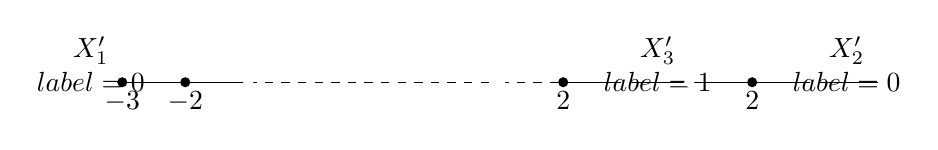
\begin{tikzpicture}[scale=0.8]
    % Draw the first segment
    \draw (-3,0) -- (-2,0);
    \draw (-2,0) -- (-1,0);
    \draw[dashed] (-1,0) -- (3,0);
    
    % Mark points on the first segment
    \filldraw[black] (-3,0) circle (2pt) node[anchor=north] {$-3$};
    \filldraw[black] (-2,0) circle (2pt) node[anchor=north] {$-2$};
    \filldraw[white] (-1,0) circle (2pt) node[anchor=north] {$-1$};
    
    % Label the first segment
    \node at (-3.5,0.5) {$X'_1$};
    \node at (-3.5,0) {$\text{label}=0$};
    
    % Draw the second segment
    \draw[dashed] (3,0) -- (4,0);
    \draw (4,0) -- (5,0);
    \draw (5,0) -- (6,0);
    
    % Mark points on the second segment
    \filldraw[white] (3,0) circle (2pt) node[anchor=north] {$1$};
    \filldraw[black] (4,0) circle (2pt) node[anchor=north] {$2$};
    \filldraw[white] (5,0) circle (2pt) node[anchor=north] {$3$};
    
    % Label the second segment
    \node at (5.5,0.5) {$X'_3$};
    \node at (5.5,0) {$\text{label}=1$};
    
    % Draw the third segment
    \draw (6,0) -- (7,0);
    \draw (7,0) -- (8,0);
    \draw (8,0) -- (9,0);
    
    % Mark points on the third segment
    \filldraw[white] (6,0) circle (2pt) node[anchor=north] {$1$};
    \filldraw[black] (7,0) circle (2pt) node[anchor=north] {$2$};
    \filldraw[white] (8,0) circle (2pt) node[anchor=north] {$3$};
    
    % Label the third segment
    \node at (8.5,0.5) {$X'_2$};
    \node at (8.5,0) {$\text{label}=0$};
\end{tikzpicture}

\end{document}